\documentclass[tikz,border=10pt]{standalone}
\usepackage{pgfplots}
\pgfplotsset{compat=1.16}

\begin{document}
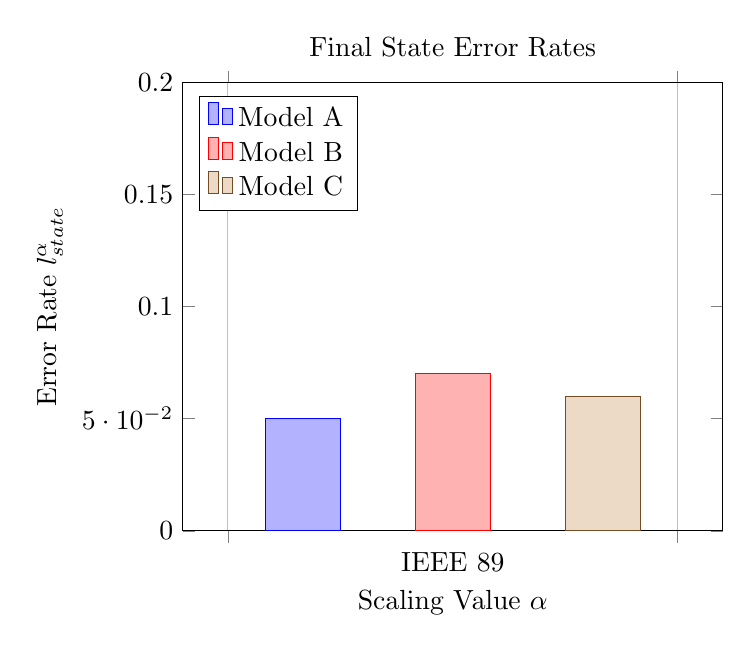
\begin{tikzpicture}
    \begin{axis}[
        title={Final State Error Rates},
        xlabel={Scaling Value $\alpha$},
        ylabel={Error Rate $l_{\text{state}}^\alpha$},
        legend pos=north west,
        ybar interval=0.5,
        symbolic x coords={IEEE 89, IEEE 118},
        xtick=data,
        ymin=0,
        ymax=0.2,
        bar width=20pt
    ]
        \addplot coordinates {(IEEE 89, 0.05) (IEEE 118, 0.03)};
        \addlegendentry{Model A}
        
        \addplot coordinates {(IEEE 89, 0.07) (IEEE 118, 0.04)};
        \addlegendentry{Model B}
        
        \addplot coordinates {(IEEE 89, 0.06) (IEEE 118, 0.05)};
        \addlegendentry{Model C}
    \end{axis}
\end{tikzpicture}
\end{document}